\section{Modeling a Realistic Manufacturing Testbed}
\label{sec:smart}

To  demonstrate the expressive power of our modeling framework we present a formal model of the System-level Manufacturing and Automation Research Testbed (SMART), a realistic testbed at the University of Michigan.

\subsection{SMART System Overview}
\label{subsec:smart_overview}
SMART is a hybrid serial-parallel line manufacturing testbed at University of Michigan~\cite{ilya:smart} (see Figure~\ref{fig:smart_layout}). It has three cells and two conveyor lines connected with a controllable pneumatic diverter. There are three industrial robots and four CNC milling machines that can produce discrete products.

Blocks 1 and 2 each contain two CNC machines and a six degree of freedom robotic arm.
Each of the CNCs are controlled by a PLC and are pre-programmed to perform operations based on the inputs from central controller (in our model, the central controller is the baseline controller). The robotic arm is programmed to pick and place parts between the conveyor and the CNCs one at a time. Blocks 1 and 2 are linked with a single conveyor line. The conveyor from Block 2 branches out into two separated conveyors going to Blocks 1 and 3. There is a diverter at the conveyor fork that determines which branching conveyor a widget takes. Block 3 contains the last robotic arm in the system that is used for additive manufacturing.

The SMART system has various sensors for gathering plant and widget state information. A camera system captures images of the widgets. 
%The widgets are carried by pallets moving around on the testbed via the conveyor system.
There are RFID transceivers and seven proximity sensors installed for locating widgets.
Each widget is  labeled with a unique RFID tag and  ID. 
The RFID tags have re-write capabilities, which can be used to store operation data such as the $\completed{}$ variable. 
%All six RFID transceivers are able to read and write data for each tag.
%SMART collects all possible data flowing in the plant.
%Besides the working part information detected and read by the proximity sensors and RFID transceivers, operational data is also recorded.
For each CNC, the motor's position for each axis and the load on the motor are captured.
For each robotic arm, the position of the joints and end effector are obtained from the robot controller.
Energy consumption of SMART is also measured and recorded for the conveyors, robotic arms and one of the CNCs.  
The collected data is sent to the central controller.
% configure PLC logic.


\begin{figure}[t]
%\vspace{-\baselineskip}
\centering
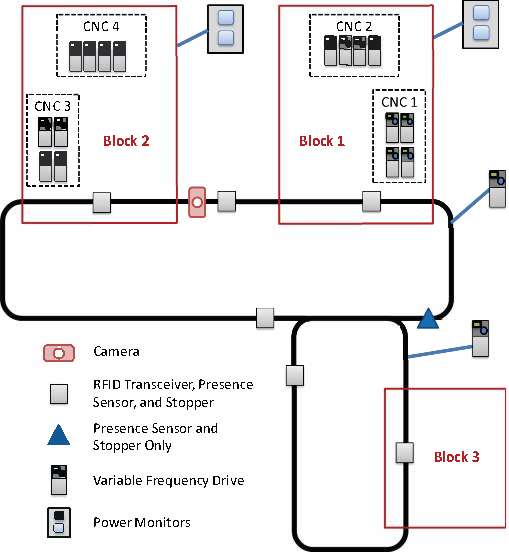
\includegraphics[width=0.7\columnwidth]{Figures/SMART_layout}
%\vspace{-\baselineskip}
\caption{\small Layout of the SMART testbed.}
\label{fig:smart_layout}
%\vspace{-1\baselineskip}
\end{figure}

\begin{figure}[t]
%\vspace{-\baselineskip}
\centering
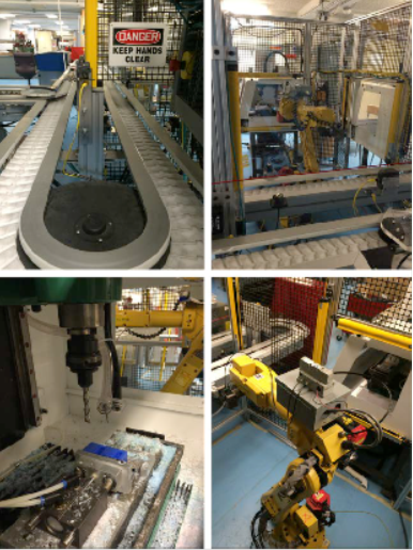
\includegraphics[width=0.6\columnwidth]{Figures/SMART_photos}
%\vspace{-\baselineskip}
\caption{\small Machine cells and conveyors.}
\label{fig:smart_photos}
%\vspace{-1\baselineskip}
\end{figure}



\begin{figure}[t]
	\begin{center}
		\resizebox{0.4\textwidth}{!}{%
		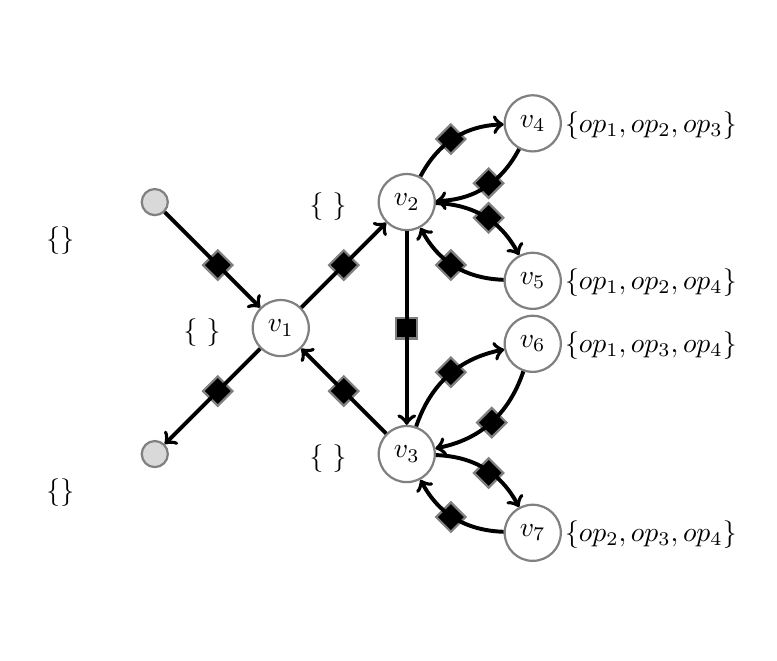
\begin{tikzpicture} 
			%[scale=.8,auto=left,every node/.style={circle,fill=blue!20}]
            [scale=.8,auto=left,every node/.style={circle,draw=black!50, thick},every path/.style={line width=0.5mm}]
            
%			\node[circle, fill=gray!30, label={[xshift=-1.2cm, yshift=-1.1cm, align=left]$\{\optop\}$\\test 2nd line}] (v_o) at (-3,2) {$\verttop$};
			\node[circle, fill=gray!30, label={[xshift=-1.2cm, yshift=-1.1cm, align=left]$\{\optop\}$}] (v_o) at (-3,2) {$\verttop$};
            \node[circle, fill=gray!30, label={[xshift=-1.2cm, yshift=-1.1cm]$\{\opbot\}$}] (v_u) at (-3,-2) {$\vertbot$};
            
            \node[label={[xshift=-1cm, yshift=-0.9cm]$\{\ \}$}] (v_1) at (-1,0) {$v_1$};
			\node[label={[xshift=-1cm, yshift=-0.9cm]$\{\ \}$}] (v_2) at (1,2) {$v_2$};
			\node[label={[xshift=-1cm, yshift=-0.9cm]$\{\ \}$}] (v_3) at (1,-2) {$v_3$};
            
            \node[label={[xshift=1.5cm, yshift=-1.65cm]$\{op_1,op_2,op_3\}$}] (v_4) at (3,3.25) {$v_4$};
            \node[label={[xshift=1.5cm, yshift=-1.65cm]$\{op_1,op_2,op_4\}$}] (v_5) at (3,0.75) {$v_5$};
            \node[label={[xshift=1.5cm, yshift=-1.65cm]$\{op_1,op_3,op_4\}$}] (v_6) at (3,-0.25) {$v_6$};
            \node[label={[xshift=1.5cm, yshift=-1.65cm]$\{op_2,op_3,op_4\}$}] (v_7) at (3,-3.25) {$v_7$};
			

		\node[rectangle,fill=black,minimum size=7.5pt,rotate=45] (v_c) at (-2,1) {};				\node[rectangle,fill=black,minimum size=7.5pt,rotate=45] (v_c) at (0,1) {};
		\node[rectangle,fill=black,minimum size=7.5pt,rotate=45] (v_c) at (-2,-1) {};				\node[rectangle,fill=black,minimum size=7.5pt,rotate=45] (v_c) at (0,-1) {};
		\node[rectangle,fill=black,minimum size=7.5pt] (v_c) at (1,0) {};
		
		\node[rectangle,fill=black,minimum size=7.5pt,rotate=45] (v_c) at (1.7,-0.7) {};	
		\node[rectangle,fill=black,minimum size=7.5pt,rotate=45] (v_c) at (1.7,1) {};
		\node[rectangle,fill=black,minimum size=7.5pt,rotate=45] (v_c) at (1.7,3) {};
		\node[rectangle,fill=black,minimum size=7.5pt,rotate=45] (v_c) at (1.7,-3) {};
		
		\node[rectangle,fill=black,minimum size=7.5pt,rotate=45] (v_c) at (2.3,2.3) {};
		\node[rectangle,fill=black,minimum size=7.5pt,rotate=45] (v_c) at (2.3,-2.3) {};
		
		\node[rectangle,fill=black,minimum size=7.5pt,rotate=45] (v_c) at (2.3,1.75) {};
		\node[rectangle,fill=black,minimum size=7.5pt,rotate=45] (v_c) at (2.35,-1.5) {};		
						
			\path (v_o) edge[->] (v_1);
            \path (v_1) edge[->] (v_u);
			\path (v_1) edge[->] (v_2);
			\path (v_2) edge[->] (v_3);
            \path (v_3) edge[->] (v_1);
            \path[]
            	(v_2) edge[<-,bend right] (v_4)
                (v_2) edge[->,bend left] (v_4);
            \path[]
            	(v_2) edge[<-,bend right] (v_5)
                (v_2) edge[->,bend left] (v_5);
			\path[]
            	(v_3) edge[<-,bend right] (v_6)
                (v_3) edge[->,bend left] (v_6);
            \path[]
            	(v_3) edge[<-,bend right] (v_7)
                (v_3) edge[->,bend left] (v_7);                
       
		\end{tikzpicture}
	}
	\end{center}
	\caption{\small The graph representation of SMART for the formal model.}
	\label{plantgraph}
\end{figure}


\subsection{Modeling SMART System}
\label{subsec:smart_setup}
%The case study is constructed based on SMART.
A discrete transition system model $\dst$ for SMART is obtained once we specify the  plant, a controller, and a requirement. We will use the baseline controller for this demonstration. 

In order to create the plant model for SMART, we consider Block 3 as the place where widgets enter and leave the plant (there are two product bins, one with raw parts and another with finished part).
The robotic arm in Block 3 picks a raw part from the corresponding product bin and places it on the conveyor to introduce a new part to the plant.
This corresponds to the creation of a new widget at a source node. 
A finished part has to reach Block 3 where the robotic arm picks the part from the conveyor and places it into the finish part's product bin. This sequence of actions corresponds to a part being consumed.
%
Since in our model source and sink vertices have to be distinct, we  use two separate vertices $\verttop$ and $\vertbot$  in the plant graph $G_P$ (see Figure~\ref{plantgraph}). 
In practice, this corresponds to logically splitting the Segment into two cells.
%start node and end node.
%
%creation of a new widget at a source node. 
%We assume there is no limit in space for the product bins.
%
Since all four CNCs can perform operations in parallel, we model each of the CNCs as a single cell in $G_P$.
There are four different operations $(\OP)$, listed in Table~\ref{tab:smart_operation_time}.
%We assume that parts are queued on the conveyors.
\begin{table}[!t]
\centering
\caption{\small Time $T_P$ for each CNC machine to complete operations.}
\label{tab:smart_operation_time}
\begin{tabular}{|c|c|c|c|c|}
\hline 
 & CNC 1 ($v_4$) & CNC 2 ($v_5$) & CNC 3 ($v_6$) & CNC 4 ($v_7$) \\ 
\hline \hline
$op_1$ & 20 & 25 & 35 & -- \\ 
\hline 
$op_2$ & 50 & 30 & -- & 10 \\ 
\hline 
$op_3$ & 25 & -- & 15 & 30 \\ 
\hline 
$op_4$ & -- & 10 & 25 & 30 \\ 
\hline 
\multicolumn{5}{l}{* all values are scaled to transition time ticks} \\
\multicolumn{5}{l}{* ``--'' indicates that the operation is not supported on this machine}
\end{tabular} 
\end{table}

\begin{table}[!t]
\centering
\caption{Operation requirements. Three requirements are considered in the case study in SMART.}
\label{tab:smart_requirements}
\begin{tabular}{|c|l|}
\hline
 & \multicolumn{1}{c|}{Operations}            \\ \hline \hline
$R_1$         & $\optop \ra op_1 \ra op_2 \ra op_3 \ra op_4 \ra \opbot$ \\ \hline
$R_2$         & $\optop \ra op_1 \ra op_3 \ra op_1 \ra \opbot$  \\ \hline
$R_3$         & $\optop \ra op_2 \ra (op_3\ , \ op_4) \ra op_1 \ra \opbot$  \\ \hline
\end{tabular}
\end{table}    

%\subsection{Formal Model}
%\cy{To be finished.}

The robot arms and the diverter act as forks in the plant that allow widgets travel along any of the forking paths. To capture this behavior, they are modeled as cells that only perform a $\noop$ operation.



Consider three types of widgets to be fabricated on SMART.
The requirement for each widget type is given in Table~\ref{tab:smart_requirements}.
The symbol ``--'' indicates that the operation is not supported by the corresponding CNC machine in that column.

Requirement 1 ($R_1$) is a typical manufacturing process that requires a sequence of different operations.
In this case, all four operations have to be performed in the given order for this type of widgets.
Requirement 2 ($R_2$) is a slightly different process. 
It is comprised of two types of operations but requires $op_1$ to be revisited in the end.
%This is common 
Requirement 3 ($R_3$) shows a more variant process.
The first operation in $R_3$ is mandatory.
 	